\begin{figure}[H]
\centering
  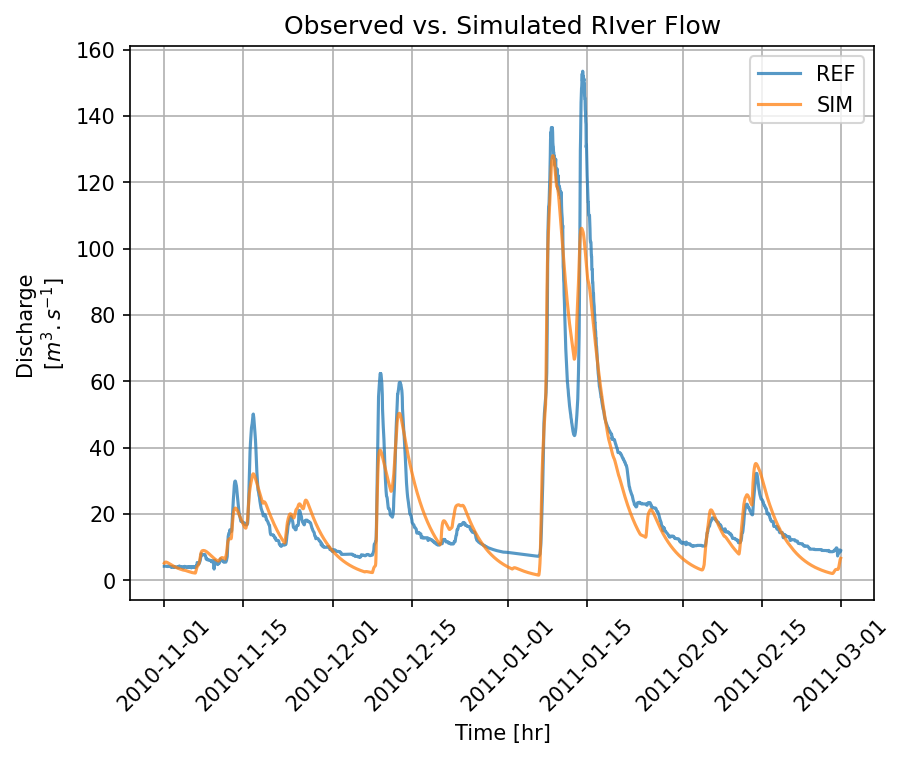
\includegraphics[width=0.8 \textwidth]{Figures/Ass_01/reworked/observed_vs_simulated_best.png}
    \caption{Discharge for optimized model Parameters with NSE = 0.908}
    \label{fig: dis_gen600}
\end{figure}

Initial runs with 600 generations and a population size of 10 yielded the best result with a very good \ac{nse} of 0.908 (rounded up) (fig:\ref{fig: dis_gen600}). Due to the stop criterion (number of significant decimals), the \ac{de} stopped after 419 generations. As seen in figure \ref{dev_ofv_gen}, the development of the best \ac{ofv} (running best (min)) decreases very slightly after 100 generations. A more detailed look at the development of each \ac{mp} (fig: \ref{fig: total_cov}) shows that some \ac{mp} approaches a narrow \ac{mp} value range after a number of generations, which is an indicator of sensitive \ac{mp}. Others, for example, urr\_tdh, with continuously high fluctuations, are not sensitive. Table \ref{tab:range_conv} ranks the \ac{mp}, which approaches a certain value. In total, 8 parameters were identified, with the latest approach around 250 germination. This seems to be the minimum number of generations needed without changing the other settings to achieve a very good result while minimizing computation time. Two test runs with 250 generations yielded very good \ac{nse} values of 0.905 and 0.907, confirming the assumption. Even if the \ac{de} algorithm were run with the same settings and inputs, the results would differ slightly at the third decimal place but would still be considered equally good. 

\begin{figure}[H]
    \centering
    \begin{minipage}[t]{0.48\textwidth}
        \centering
        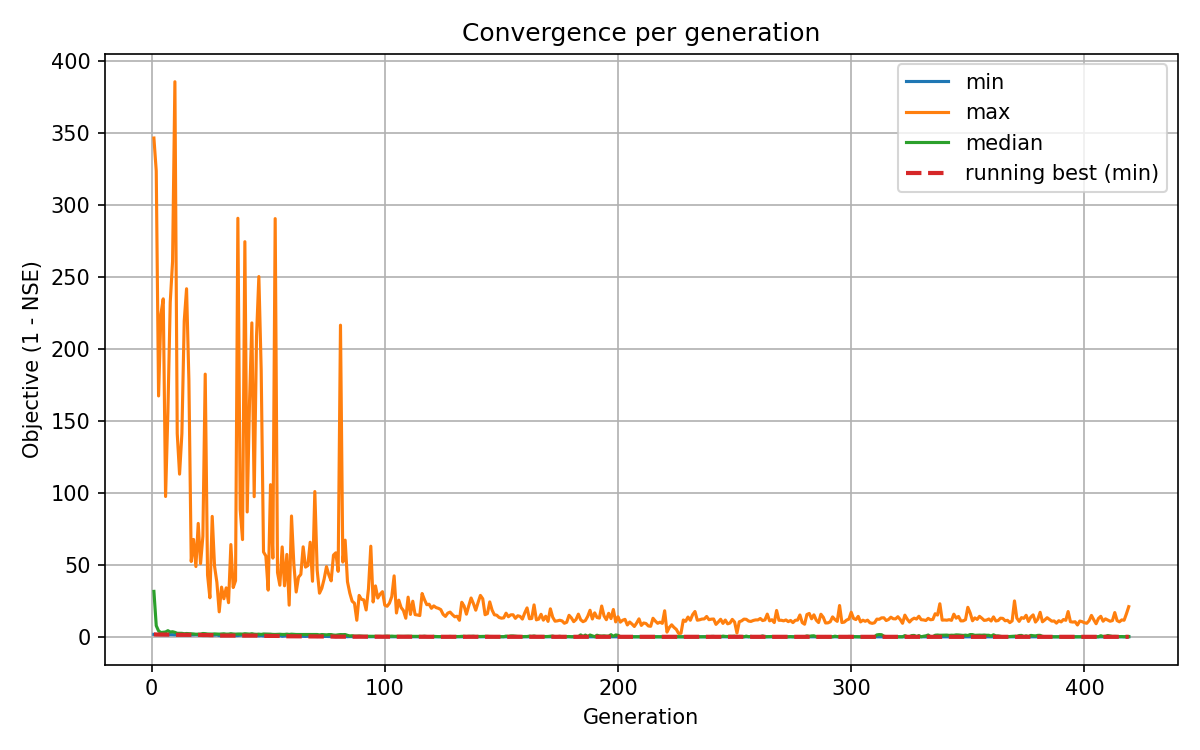
\includegraphics[width=\textwidth]{Figures/Ass_01/reworked/convergence_per_generation_ytotal.png}
        %\caption{Irr\_dre}
        %\label{fig:irr_dre}
    \end{minipage}
    \hfill
    \begin{minipage}[t]{0.48\textwidth}
        \centering
        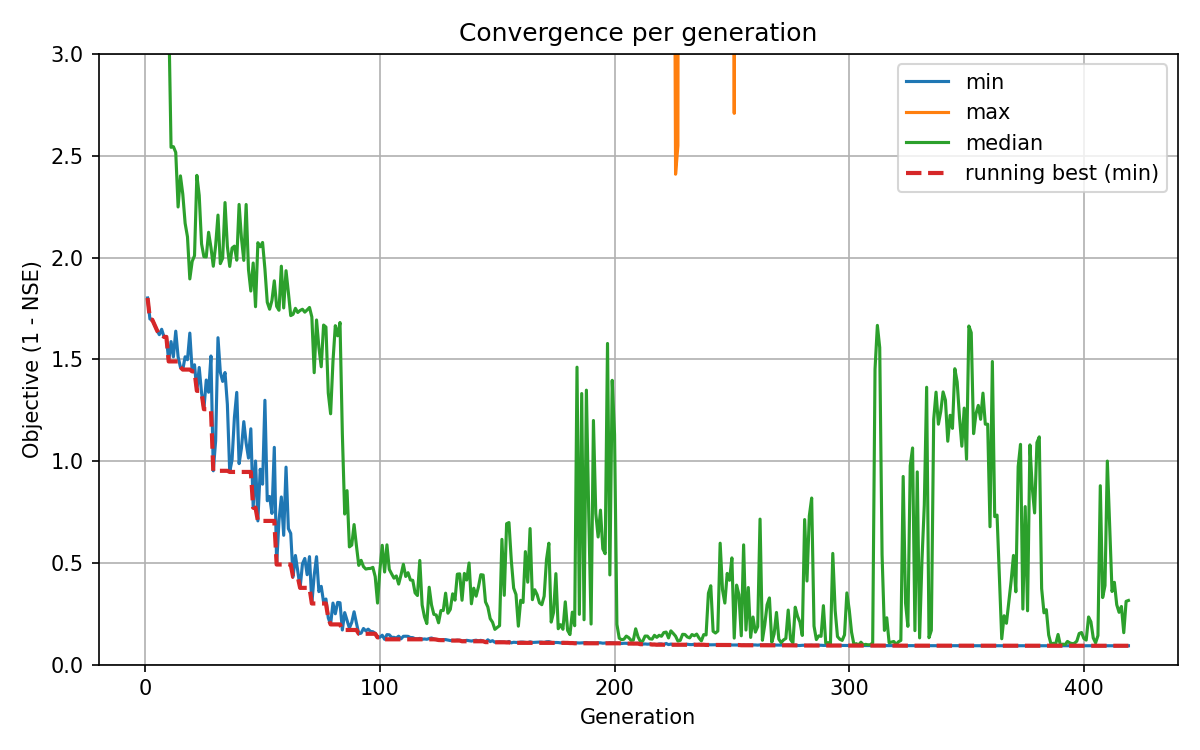
\includegraphics[width=\textwidth]{Figures/Ass_01/reworked/convergence_per_generation.png}
    \end{minipage}
    \caption{Development of OFV for each generation (right: zoom in)}
    \label{dev_ofv_gen}
\end{figure}

\begin{figure}[H]
\centering
  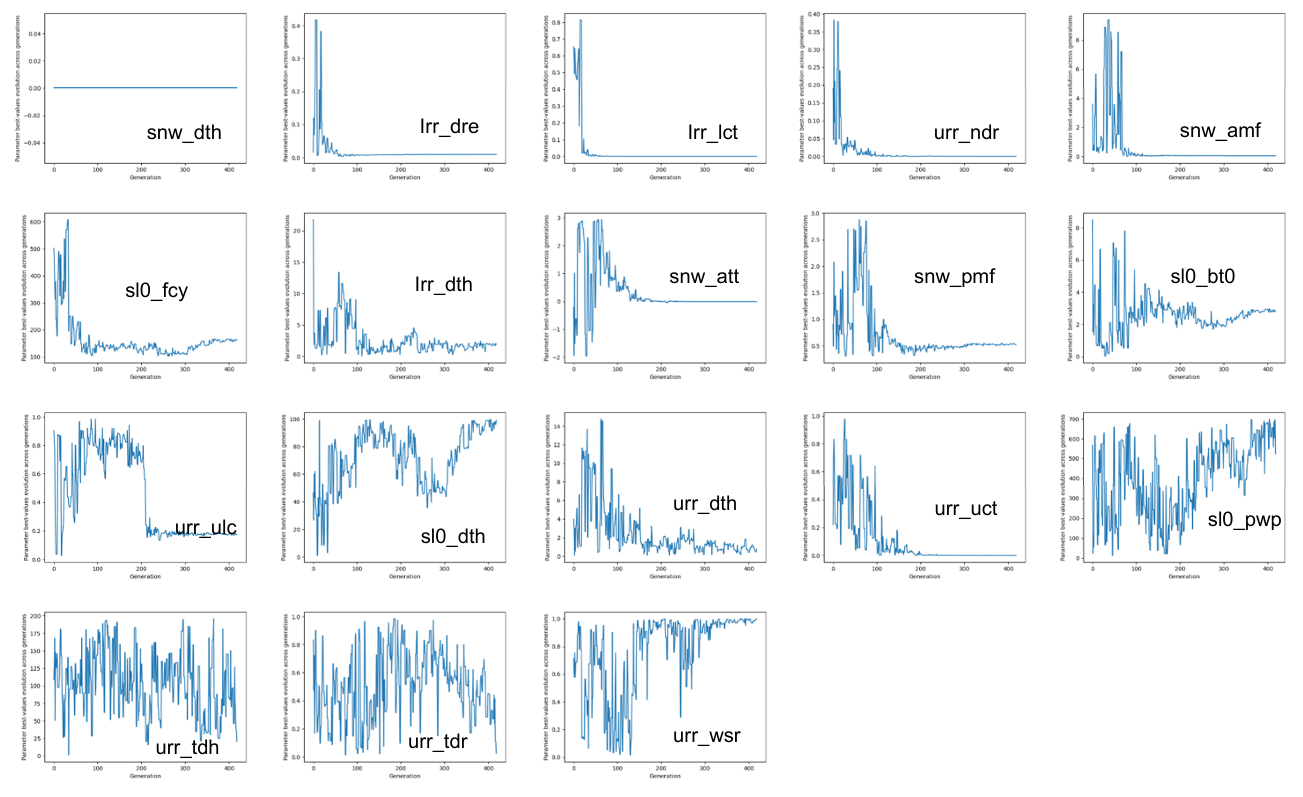
\includegraphics[width=1 \textwidth]{Figures/Ass_01/reworked/MP_dev_total_gen600.png}
    \caption{overview of convergence of all MP}
    \label{fig: total_cov}
\end{figure}

\begin{table}[H]
\centering
\begin{tabular}{ccc}
\hline
Ranking & ac{mp} & around generation \\ \hline
1 & Irr\_lct & 80  \\
2 & Irr\_dre & 100  \\
3 & snw\_amf & 130  \\
4 & urr\_ndr & 180  \\ 
5 & snw\_att & 200  \\
5 &  urr\_uct & 200  \\ 
6 & snw\_pmf & 250  \\ 
6 & urr\_ulc & 250  \\ \hline
\end{tabular}
\caption{ranking convergence of MP}
\label{tab:range_conv}
\end{table}

Notably, only the percolation ratio, \ac{mp}, urr\_ulc shows a sudden value shift around 200 generations (fig: \ref{urr_ulc}). This indicates that the \ac{de} changes the solution area, from a local maximum or a second global maximum. In a test run with 180 generations, this occurrence disappears, achieving a very good \ac{nse} of 0.893. 

\begin{figure}[H]
    \centering
    \begin{minipage}[t]{0.45\textwidth}
        \centering
        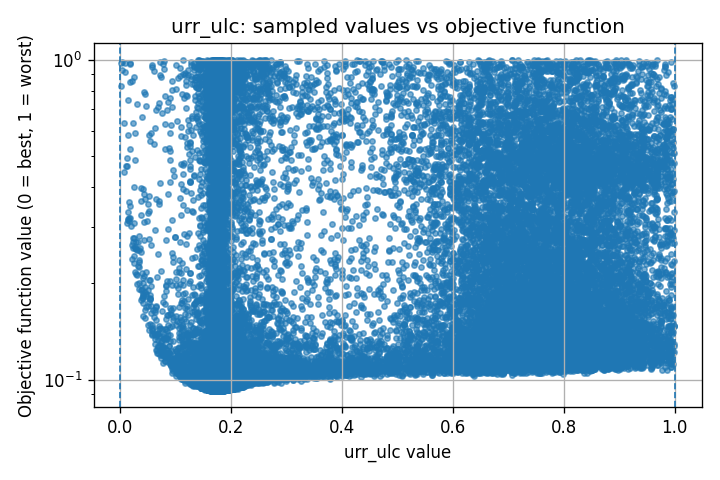
\includegraphics[width=\textwidth]{Figures/Ass_01/reworked/param_scatter_urr_ulc.png}
        %\caption{Irr\_dre}
        %\label{fig:irr_dre}
    \end{minipage}
    \hfill
    \begin{minipage}[t]{0.45\textwidth}
        \centering
        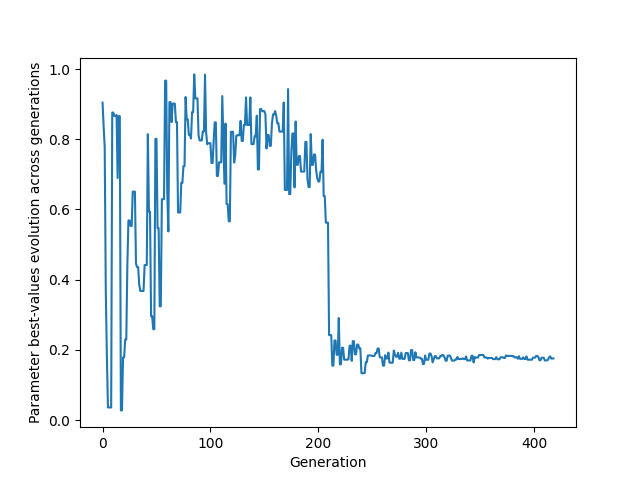
\includegraphics[width=\textwidth]{Figures/Ass_01/reworked/params_evolution_per_generation_urr_ulc.png}
    \end{minipage}
    \caption{urr\_ulc}
    \label{urr_ulc}
\end{figure}

In the scatter plots, the \ac{mp} values (log-scale) are plotted against the reached $\ac{ofv} \le 1$. The snow depth is fixed at zero and can be ignored. A spike-like and narrow point cloud is an indicator for sensitive \ac{mp} (fig: \ref{fig: total_sc}). Concerning these two aspects, four categories are identified: very narrow total parameter range and taper (e.g. Irr\_dre); full range but narrowing fast, with differences in the range of the best \ac{ofv} (e.g. snw\_att and sl0\_bt0); wide range for most of the \ac{ofv} with a more narrow range for the best \ac{ofv} (e.g. urr\_tdh); and full range for all \ac{ofv} (e.g. urr\_wst). Not sensitive \ac{mp} are very clear identified: sl0\_pwp, urr\_tdh, urr\_ tdr, and urr\_wsr. For the others, based solely on the scatter plots, a ranking above the categorization is vague. The convergence of the \ac{mp} (tab: \ref{tab:range_conv}) is used for further sorting within the categories in figure \ref{fig: total_sc} (read from left to right). 

\begin{figure}[H]
\centering
  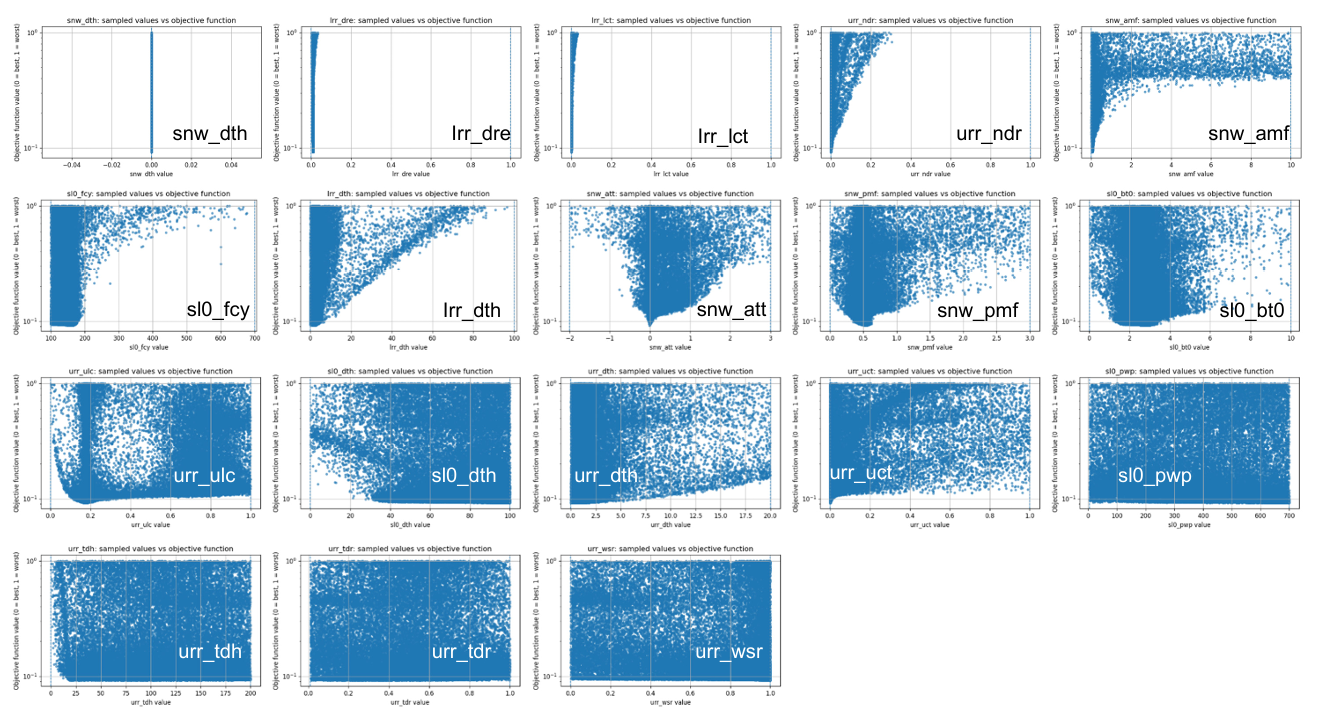
\includegraphics[width=0.9 \textwidth]{Figures/Ass_01/reworked/scatter_total_gen600.png}
    \caption{overview of all scatter plots}
    \label{fig: total_sc}
\end{figure}

\newpage
\textbf{turning off Processes}

\begin{figure}[H]
    \centering
    \begin{minipage}[t]{0.45\textwidth}
        \centering
        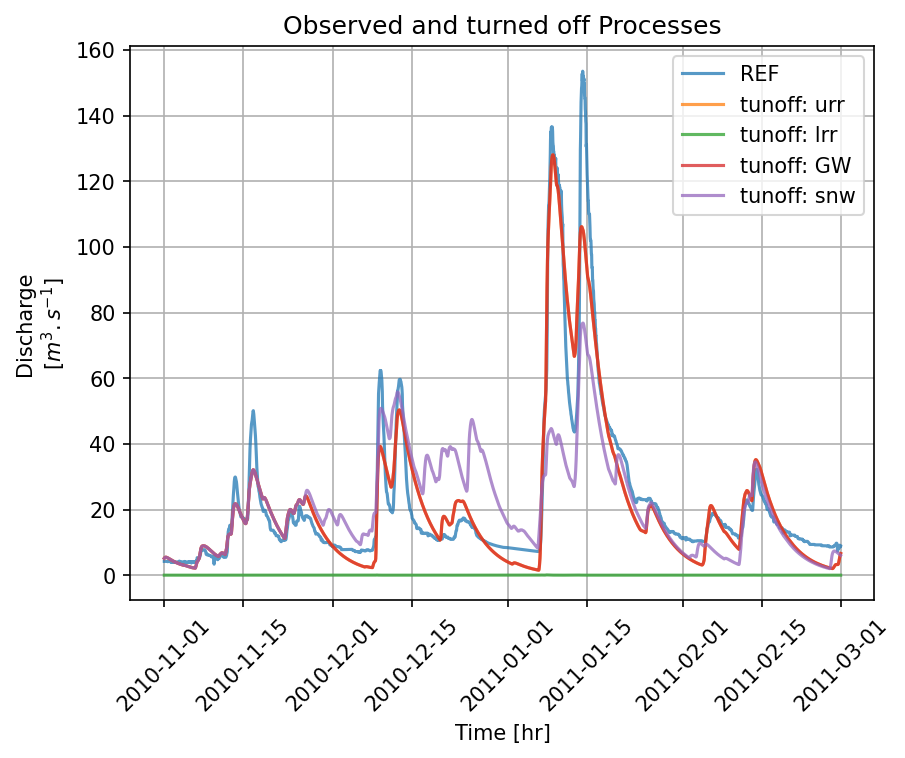
\includegraphics[width=\textwidth]{Figures/Ass_01/turnoff/observed_with_turnoff.png}
        %\caption{Irr\_dre}
        %\label{fig:irr_dre}
    \end{minipage}
    \hfill
    \begin{minipage}[t]{0.45\textwidth}
        \centering
        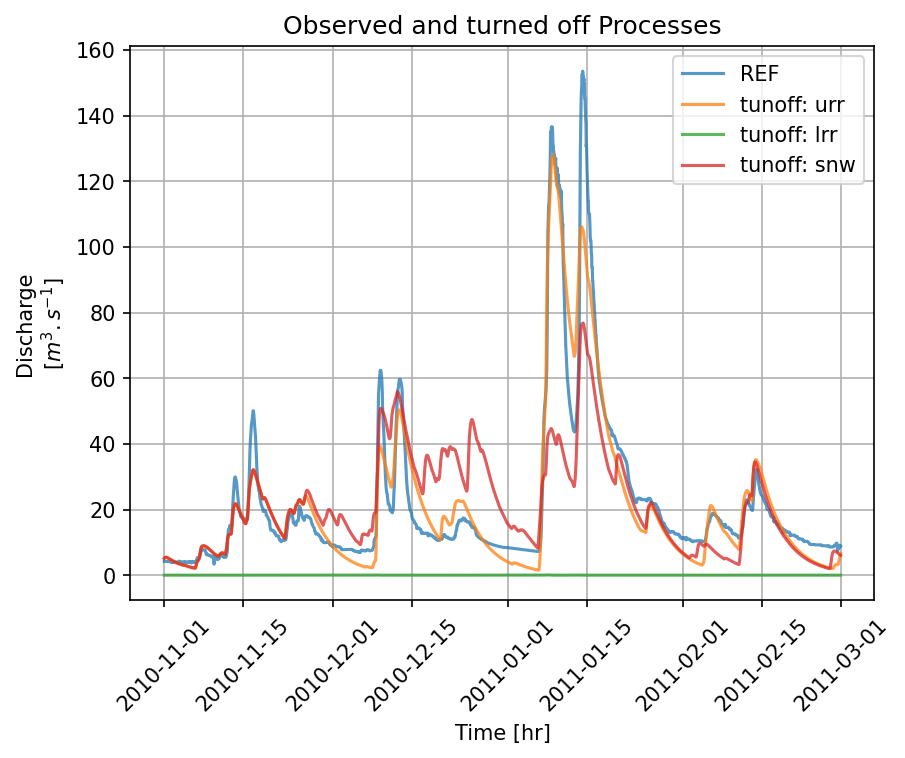
\includegraphics[width=\textwidth]{Figures/Ass_01/turnoff/observed_with_turnoff_withoutGW.png}
    \end{minipage}
    \caption{Comparison turned off Processes with observed discharge}
    \label{fig: turnedoff_Proc}
\end{figure}

Turning off the \ac{gw} flow and the upper reservoir processes resulted in identical hydrographs (fig: \ref{fig: turnedoff_Proc} and \ref{fig: dis_gen600}) and in a \ac{nse} = 0.908. Due to the very slow flow of \ac{gw}, it is expected to contribute only small amounts to the water balance. The contribution would accumulate over a long period, but the observed time period is very short. No changes during the turned-off upper reservoir process indicate that the model is using only the lower reservoir, as confirmed by the results from the turned-off lower reservoir. This concludes that the model does not rely on the use of the entire module to simulate this very short time period with only one high-flow peak event. Running the \ac{de} algorithm again to find the optimal \ac{mp} with the lower reservoir parameter turned off resulted in \ac{nse}=0.900, indicating that the model can compensate using the upper reservoir. The turned-off snow process (\ac{nse} = 0.496) shows the strong influence of the snow on the high peak event and the prior cold period (fig: \ref{fig: turnedoff_snw}, \ref{fig: turnedoff_Proc}). 

\begin{figure}[H]
    \centering
    \begin{minipage}[t]{0.45\textwidth}
        \centering
        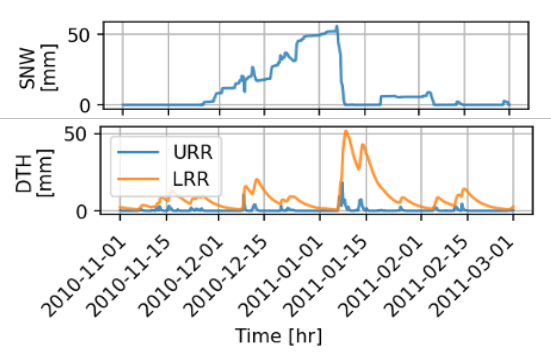
\includegraphics[width=\textwidth]{Figures/Ass_01/turnoff/unchanged.PNG}
        %\caption{Irr\_dre}
        %\label{fig:irr_dre}
    \end{minipage}
    \hfill
    \begin{minipage}[t]{0.45\textwidth}
        \centering
        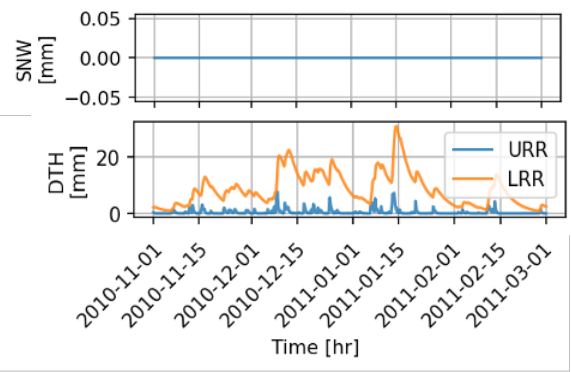
\includegraphics[width=\textwidth]{Figures/Ass_01/turnoff/snw_turn_off.PNG}
    \end{minipage}
    \caption{Comparison of no turned-off processes (left) with turned off snow Processes (right) }
    \label{fig: turnedoff_snw}
\end{figure}

\begin{comment}
NSE without change = 0.9076084494590759
NSE_urr = 0.90763258934021
NSE_lrr = -0.7538880109786987
NSE_snw = 0.4959281086921692


    
\begin{figure}[H]
    \centering
    \begin{minipage}[t]{0.48\textwidth}
        \centering
        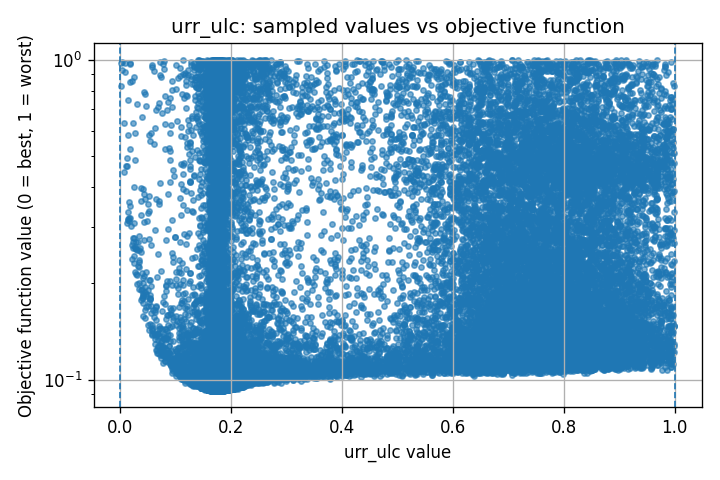
\includegraphics[width=\textwidth]{Figures/Ass_01/reworked/param_scatter_urr_ulc.png}
        %\caption{Irr\_dre}
        %\label{fig:irr_dre}
    \end{minipage}
    \hfill
    \begin{minipage}[t]{0.48\textwidth}
        \centering
        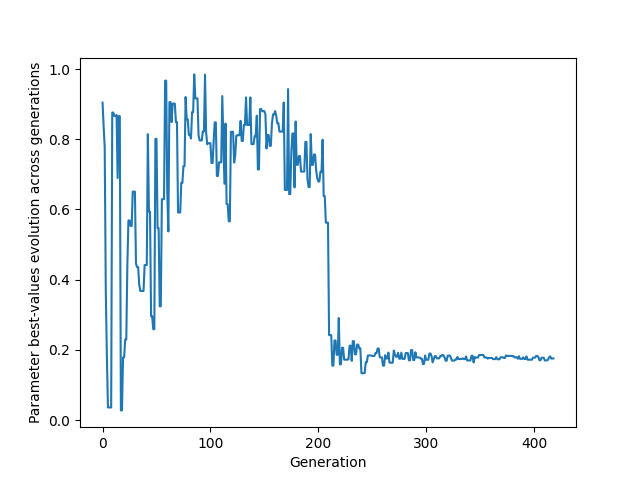
\includegraphics[width=\textwidth]{Figures/Ass_01/reworked/params_evolution_per_generation_urr_ulc.png}
        
    \end{minipage}
    
    \vspace{0.5cm}
    
    \begin{minipage}[t]{0.48\textwidth}
        \centering
        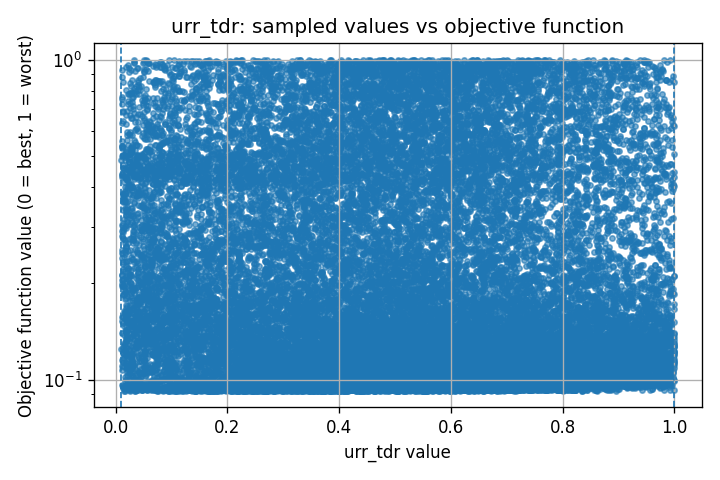
\includegraphics[width=\textwidth]{Figures/Ass_01/reworked/param_scatter_urr_tdr.png}
    \end{minipage}
    \hfill
    \begin{minipage}[t]{0.48\textwidth}
        \centering
        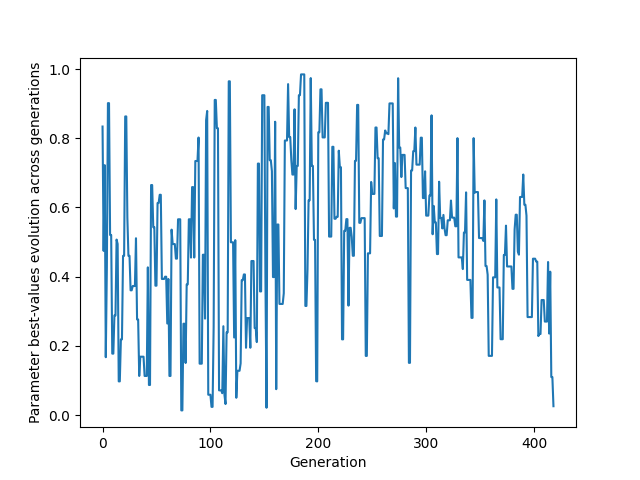
\includegraphics[width=\textwidth]{Figures/Ass_01/reworked/params_evolution_per_generation_urr_tdr.png}
    \end{minipage}
    \caption{model parameter vs objective function, narrow range}
    \label{fig: width range}
\end{figure}

\end{comment}



\begin{comment}
• Obtain best performing parameter vector
• Estimate the least number of processes
required
− Similar overall efficiency
− Makes physical sense
• Plot internal model variables
− With all processes turned on
− With some turned off
• Plot convergence of the OFVs
• Plot parameter vs. OFVs (each)
− Can you tell which ones are sensitive?

turn off Processes 
\end{comment}